%!TEX root = ../main-anran-ma.tex 
% so I can build in this tex file too. 
%************************************************
% \setcounter{theorem}{6}
\chapter{Necessary Liberal Preconditions}\label{ch:nlp} % $\mathbb{ZNR}$
%************************************************

% \section{Literature Review}

% Here is a description of all the triples. 
% \todo{Literature review section}



We are interested in studying the \define{necessary liberal precondition}, a weakening of the weakest liberal precondition: 
$$wlp.C.F\implies G$$
We show our interest, by relating all the pre- and postcondition transformers, so we can distinguish the existing triples that are already well-researched graphically. 

Luckily, we can find scenarios where the overapproximation can be useful, and demonstrate it with an example, before giving a proof system. 
We conclude that this overapproximation can help us find more preconditions that can lead to failure, either by including states that lead to unidentified errors, or by including states that can lead to errors via non-terministic choice. 
The latter method then leads to finding conditions that are able to capture these special states. 
The side effect of this result is that we can now find the wlp transformer with angelic non-determinism using wlp with demonic non-determinism and sp.

This chapter includes our most important results: 
\begin{enumerate}
	\item The predicate transformers are all related together nicely by relations like termination, reachability, conjunction, over- and under-approximation, and implication in both directions. 
	\item Without any additional constraints, the necessary liberal preconditions can be anything. The only thing we are sure of is that its negation guarantees termination in the negation of the desired postcondition. 
	\item Necessary liberal preconditions find their usefulness in avoiding bugs. 
	\item With necessary liberal precondition, we also can overapproximate and underapproximate wlp with angelic non-determinism ($wlp_a$). In the end, we can qualify $wlp_a$ using necessary liberal precondition and strongest postcondition transformers, without having to define $wlp_a$.  
\end{enumerate}


In the upcoming sections, we first relate together wp, wlp, sp, and slp with both angelic and demonic non-determinism, so we can distinguish the necessary liberal precondition from the existing triples that are already well-studied. 
In this chapter, we first discuss the general semantics of the necessary liberal precondition, then focus on a characteristic scenario and show properties that captures it. 





\section{The General Case}\label{sec:general}
As hinted before, in our triple $wlp.C.F\implies G$, $G$ overapproximates wlp. 
It can take different forms: on the one hand, $G$ can be so general that it is satisfied by any program state; on the other hand, a $G$ that is barely weaker than $wlp.C.F$ is also not much different from the latter. 
Alternatively, $G$ can also be all kinds of preconditions that starting from it, any postcondition is reachable. 
One thing we are certain about, though, is that a program with an original state satisfying $\neg G$ will terminate, and the final state can satisfy $\neg F$: 
\begin{align*}
wlp.C.F{\implies} G & \Leftrightarrow \neg G {\implies} \neg wlp.C.F \\
	& \Leftrightarrow \neg G {\implies} wp.C.\neg F 
	\hspace{0.2\textwidth} \mid {\thm{conjugate}}
\end{align*}
These equivalences indicate that \hoare{\neg G}C{\neg F} is a valid Hoare triple with respect to total correctness, i.e. if $C$ starts in an initial condition satisfying $ \neg G$, then its execution \imptt{must} terminate, and it must be able to terminate satisfying $\neg F$. 

\subsection{Overapproximation of wlp}
In \autoref{sec:wlp} we define the weakest liberal precondition and state that it characterizes all the preconditions starting from which the program either \imptt{diverges} or \imptt{will} terminate in a state satisfying $F$. 
We are certain to use ``will'' instead of ``can'' as the non-deterministic choice is viewed as demonic, so the behavior of wlp can be depicted by \autoref{subfig:wlpd}. 

The rectangle on the left (right) denote the set of all initial (final) states $\S$. 
$C$ is the program, and its executions are depicted by arrows. 
The rectangle is divided into halves, the part with label $wlp.C.F$ denotes all the states that satisfy $wlp.C.F$, and so on. 
The dashed arrow starting from inside a rectangle, ending outside of either triangle denotes executions that do not terminate. 
The arrows that share the same point from the left rectangle denote different executions starting from the same initial state. 

Starting from one initial state, the execution of the program can take various forms: it can be strictly deterministic, or it can have multiple non-deterministic choices; it can terminate in a final state, or it can execute forever. 
We categorize the executions of the program in four ways: 
\begin{enumerate}
	\item the dashed arrow means non-terminating executions; 
	\item the black arrows are executions starting from an initial state satisfying $wlp.C.F$ and only terminating in final states satisfying $F$; 
	\item the green arrows are the executions starting from an initial state satisfying $\neg wlp.C.F$ but can terminate in states either satisfying $F$ or satisfying $\neg F$;
	\item the red arrow represents executions starting from an initial state satisfying $\neg wlp.C.F$ and only terminating in final states satisfying $\neg F$. 
\end{enumerate}


\begin{figure}[ht!]\centering
	\subfloat[Weakest liberal precondition (demonic non-determinism)\label{subfig:wlp-g}]{
		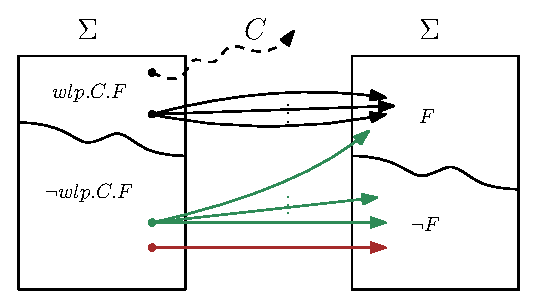
\includegraphics[width=0.4\textwidth]{image/wlp-g/wlpd.eps}}
	\hfill

	\subfloat[Precondition $G$ with $wlp.C.F\implies G$ and $G$ contains some green arrows\label{subfig:wlp-g-g}]{
		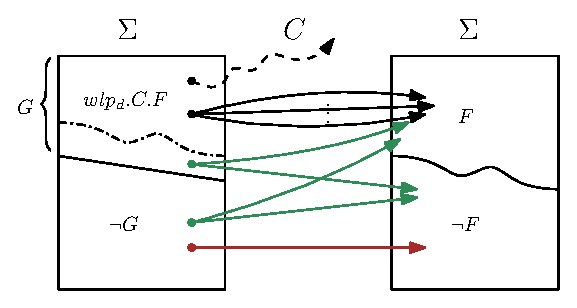
\includegraphics[width=0.45\textwidth]{image/wlp-g/wlp-g-g.eps}
	}
	\hfill
	\subfloat[Precondition $G$ with $wlp.C.F\implies G$ and $G$ contains all the green arrows\label{subfig:wlp-g-gg}]{
		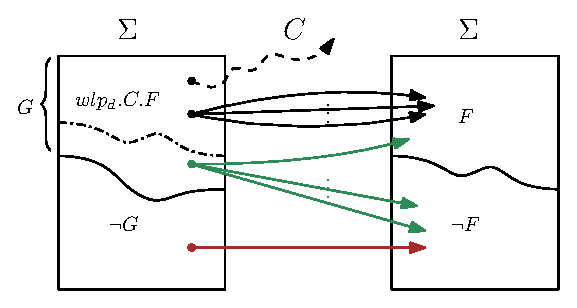
\includegraphics[width=0.45\textwidth]{image/wlp-g/wlp-g-gg.eps}
	}

	\subfloat[Precondition $G$ with $wlp.C.F\implies G$ and $G$ contains some red arrows\label{subfig:wlp-g-r}]{
		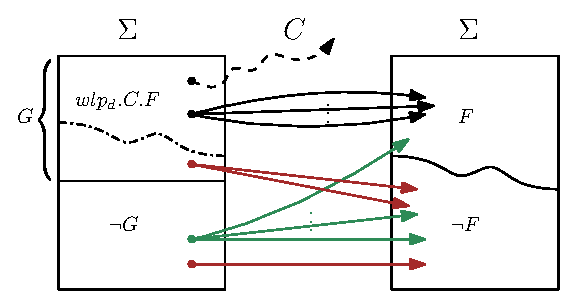
\includegraphics[width=0.45\textwidth]{image/wlp-g/wlp-g-r.eps}
	}
	\hfill
	\subfloat[Precondition $G$ with $wlp.C.F\implies G$ and $G$ contains all the red arrows\label{subfig:wlp-g-rr}]{
		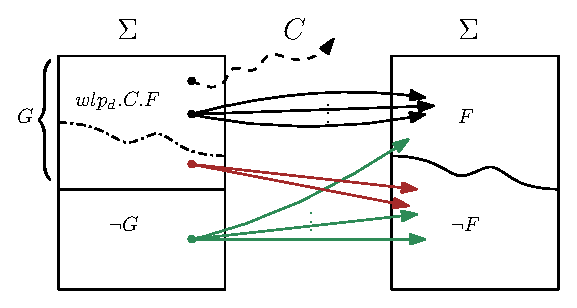
\includegraphics[width=0.45\textwidth]{image/wlp-g/wlp-g-rr.eps}
	}
\caption{Case Distinction of Preconditions Weaker Than wlp}
\label{fig:wlp-g-1}
\end{figure}

\begin{figure}[ht!]\centering
	\ContinuedFloat
	\subfloat[Precondition $G$ with $wlp.C.F\implies G$ and $G$ contains some green arrows and some red arrows\label{subfig:wlp-g-gr}]{
		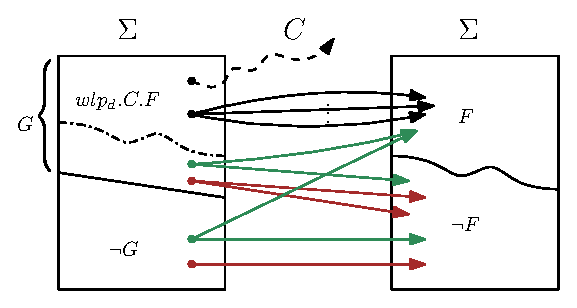
\includegraphics[width=0.45\textwidth]{image/wlp-g/wlp-g-gr.eps}
	}
	\hfill
	\subfloat[Precondition $G$ with $wlp.C.F\implies G$ and $G$ contains all the green arrows and some red arrows\label{subfig:wlp-g-ggr}]{
		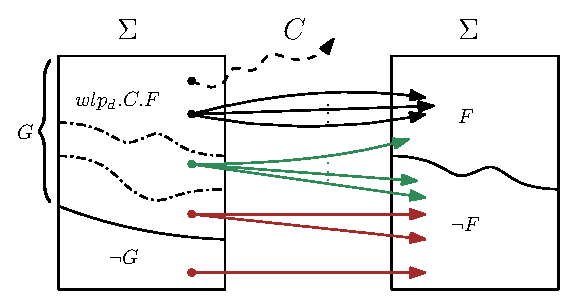
\includegraphics[width=0.45\textwidth]{image/wlp-g/wlp-g-ggr.eps}
	}

	\subfloat[Precondition $G$ with $wlp.C.F\implies G$ and $G$ contains some green arrows and all the red arrows\label{subfig:wlp-g-grr}]{
		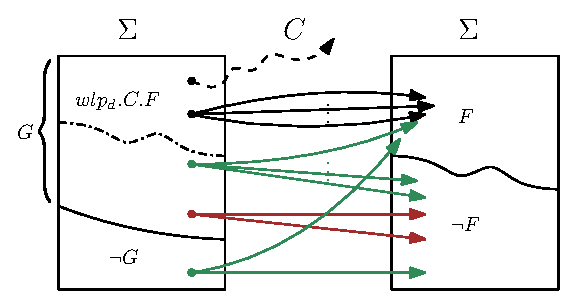
\includegraphics[width=0.45\textwidth]{image/wlp-g/wlp-g-grr.eps}
	}
	\hfill
	\subfloat[Precondition $G$ with $wlp.C.F\implies G$ and $G$ contains all the arrows\label{subfig:wlp-g-ggrr}]{
		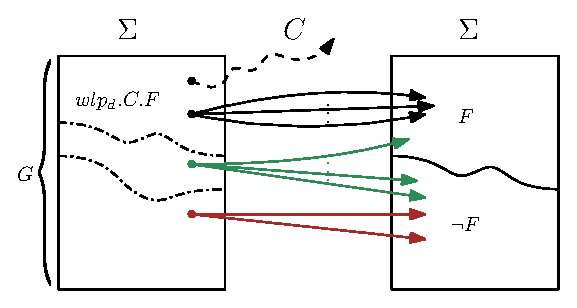
\includegraphics[width=0.45\textwidth]{image/wlp-g/wlp-g-ggrr.eps}
	}
\caption{Case Distinction of Preconditions Weaker Than wlp (Cont.) }
\label{fig:wlp-g-2}
\end{figure}
If we were to weaken the precondition, it can happen in various ways as shown in \autoref{subfig:wlpd}{\color{RoyalBlue}-9}. 
For example, \autoref{subfig:wlpd} shows the situation where $G$ is exactly $wlp.C.F$. 
But in \autoref{subfig:wlp-g-g}, $G$ is strictly weaker than $wlp.C.F$. 
Here, $G$ is satisfied by all initial states that satisfy $wlp.C.F$, plus \imptt{some} of the initial states, starting from which the execution can end satisfying $F$ or $\neg F$, aka some of the green arrows. 
Further, the $G$ in \autoref{subfig:wlp-g-gg} is satisfied by \imptt{all} the above initial states, i.e. all the green arrows start from $G$. 
The same principle applies to the red arrows. 
\autoref{subfig:wlp-g-r} shows a $G$ that is satisfied additionally by \imptt{some} of the initial states that are starting points of the red arrows, i.e. executions that start in $\neg wlp.C.F$, and end in $\neg F$. 
In \autoref{subfig:wlp-g-rr}, $G$ contains all such initial states. 

The situation can be trickier, for example in \autoref{subfig:wlp-g-gr}, $G$ is also the starting point of both green and red arrows. 
In other words, if $C$ starts from some initial state satisfying this $G$, then maybe its execution diverges, maybe it terminates satisfying $F$, maybe not. 
The same can be said about the $G$ in \autoref{subfig:wlp-g-ggr} and \autoref{subfig:wlp-g-grr}. 
Finally, $G$ is weakened so much that it is simply $true$, hence satisfied by all initial states as seen in \autoref{subfig:wlp-g-ggrr}. 

% We thus first investigate this special case, before proceeding with $G$ in general. 

% While having restrictions on $G$ yields interesting results, without the restrictions we can still find useful characteristics. 
In general, when $wlp.C.F\implies G$, $G$ can be satisfied by all possible initial states, which can be the starting points of black, green, red, or dashed arrows, representing executions terminating in states satisfying $F$, $F$ or $\neg F$, $\neg F$, or non-terminating, respectively. 
As a result, we can not make many statements without adding extra restrictions to $G$. 

However, we can see from \autoref{subfig:wlpd}{\color{RoyalBlue}-9} that when $\neg G$ is not empty, there is always some arrow ending in $\neg F$. 
So there always exists some execution that starts from an initial state satisfying $\neg G$, and ends in a final state satisfying $\neg F$%: \hoare{\neg G}C{\neg F} is a valid hoare triple. 

Alternatively, we can say that does not contain any \imptt{black} or \imptt{dashed} arrows in all cases. 
In other words, if program $C$ starts in any initial state satisfying $\neg G$, then either $G$ is empty, or
\begin{itemize}
	\item its executions terminate, and
	\item there exists an execution that ends up in a final state that satisfies $\neg F$. 
\end{itemize}

This again states that \hoare{\neg G}{C}{\neg F} is a valid Hoare triple. 
The question then naturally arises: why do we concern ourselves with $G$, if we can just prove our specifications using wp or Hoare triples? 
To demonstrate the answer, we analyze the example written in \autoref{lst:door}. 

\begin{lstlisting}[caption={Door with Sensors Counting Number of People Present}, label={lst:door}, language=java, numbers=left, stepnumber=1, captionpos=b,escapechar=|,frame=single]
	... // starting device
	n := n + 1 |$\square$| n := n - 1 |$\square$| diverge;|\label{line:tri-nondet}|
	... // retirement  
\end{lstlisting}

\subsection{Example: Door with Sensors}
In the author's student life, there was a door at university that she always finds interesting. 
The door is located at a lecture hall, equipped with two sensors on the left and right sides of the door frame. 
Each time a person walks in or out, the sensor registers and adds or decreases the number of people in the lecture hall, making a small tick sound. 
It seems that this door serves the purpose of helping security guards keep an eye on the lecture rooms after closing time without having to be physically there. 

But can the door really distinguish from a person entering or leaving the room? 
And what if naughty students try to trick the door by using a backpack to pretend to exit the door multiple times? 
What if one of the sensors break? 
We can this simple scenario by putting the three parts in non-deterministic choice. 
It can happen that a student enters the room hence increasing the count of the number of people present: $n:=n+1$; or a person exits and decreasing the number: $n:=n-1$. 
Alternatively, the sensor can break because of old age and result in unforeseeable behavior, for example always detecting someone entering forever. 

We know that there is definitely something wrong, in case the security sees on their device that the number of people in a lecture hall is negative. 
If we want to know what caused it, we can calculate the weakest liberal precondition of the program snippet with regard to $F=\{\sigma\in\S\mid\sigma.n<0\}$ in \autoref{lst:door}. 
We write $F=\{n<0\}$ in short: 
\begin{lstlisting}[caption={Weakest Liberal Precondition w.r.t Postcondition $F=\{\sigma\in\S\mid\sigma.n<0\}$ }, label={lst:neg0}, language=java, numbers=left, stepnumber=1, captionpos=b,escapechar=|,frame=single]
	... // starting device
	|\imptt{$\{n<-1\}$}|
	|\imptt{$\{n<-1\}\ \wedge\ \{n<1\}\ \wedge\ true$}|
	n := n + 1 |$\square$| n := n - 1 |$\square$| diverge;|\label{line:tri-nondet}|
	|\imptt{\{$n<0$\}}|
	... // retirement   
\end{lstlisting}

It seems like we should avoid starting the system in a state where $n$ is less than $-1$. 
But it is enough? If we start the system in a state where $n=-1$, or even $n=0$, we can still reach an erroneous state where the value of $n$ is negative. 
\autoref{fig:door}
\begin{figure}[ht]
	\centering
	\includesvg[width=0.8\linewidth]{image/example-door.svg}
	\caption{$wlp.C.F = \{n<-1\}$}
	\label{fig:door}
\end{figure}
We can see that with wlp, it is not enough to identify all preconditions that can result in errors. 
In other words, the green arrows in \autoref{fig:door} are not recognized. 
But by overapproximating wlp to include preconditions like $\{n=-1\}$ and $\{n=-1\}$, we can also include all the green arrows in $G$. 

This is, however, not the only thing that is missing. 
Obviously, a lecture hall does not have unlimited capacity. 
Once the system is showing a number higher than the maximum capacity, the security would also instantly know that something is wrong. 
Also, there could be conditions like ``during holiday time, the lecture halls are unoccupied'' that an expert of the system (the security guards in this case) would know, but not in general. 
So even by including all the green arrows via overapproximation, we are still missing some of the red arrows like in \autoref{fig:door-expert}, the hidden knowledge that seasoned users possess.   
\begin{figure}[ht]
	\centering
	\includesvg[width=0.8\linewidth]{image/example-door-expert.svg}
	\caption{$wlp.C.F \implies G$}
	\label{fig:door-expert}
\end{figure}

This demonstrates overapproximating wlp is useful to include the green and red arrows in \autoref{fig:door-expert}, aka when: 
\begin{itemize}
	\item some preconditions \imptt{can but are not guaranteed} to lead to the erroneous final states non-deterministically; 
	\item or the user only have insufficient knowledge of the system, but experts can deduce other erroneous final states that are unknown to the public. 
\end{itemize}
To utilize this overapproximation, we either identify the preconditions that result in the green arrows, which we will do in the next section, or we first calculate the weakest liberal precondition of the erroneous postcondition that we know of, then relax this precondition by ``guessing'' similar erroneous postconditions with the extra knowledge from experts over the system. 

\subsection{Example: To Exclude Bugs}
Here comes an example similar as the ones described by Cousot to overapproximate wp. 
%TODO


\subsection{Proof System}\label{sec:system}
\newcommand{\nlp}[3]{\langle #1 \rangle\ #2\ \langle #3 \rangle}
We call the overapproximation of wlp \define{necessary liberal precondition}, ``necessary'' because it is required to ensure avoidance of erroneous final states, and ``liberal'', because it is satisfied by all initial states that can potentially lead to non-termination, just like wlp. 
We provide a proof system in \autoref{tab:proof-system}. 
The rules are mostly vanilla, except from the consequence rule: 
$$\displaystyle\frac{P{\implies} G,\ \nlp P C Q,\ F{\implies} Q}{\nlp{G}{C}{F}} conseq$$
It is the complete opposite direction from the consequence rule in Hoare logic that we referred to in \autoref{tab:hoare}. 
Rewriting it in the same natural deduction style, we arrive at: 
$$\displaystyle\frac{G{\implies} P,\ \hoarenm{P}{C}{Q},\ Q{\implies} F}{\hoarenm{G}{C}{F}}conseq_h$$
This corresponds to our expectation, because we know that the overapproximation triple is exactly a Hoare triple (with respect to partial correctness) with negated pre- and postconditions:
\begin{align*}
	& \ wlp.C.F{\implies} G \\
	\Leftrightarrow &\  \neg G {\implies} \neg wlp.C.F \\
	\Leftrightarrow &\  \neg G \implies wp.C.\neg F 
		\hspace{0.3\textwidth} \mid {\thm{conjugate}} \\
	\Rightarrow &\  \hoarenm{\neg G}C{\neg F} 
	\tag{*} 
\end{align*}
Note that the last line is only an implication in one direction, because we take the version of Hoare triple regarding partial correctness, meaning that termination is not guaranteed. 
In other words, \hoare{\neg G}C{\neg F} can be a valid Hoare triple, but an initial state satisfying $\neg G$ does not necessary guarantee termination, hence $\neg G$ is not necessarily a subset of $wp.C.\neg F$. 
If we were to take Hoare triple with additional rules to prove termination~\cite{manna74}, the implication would be in both directions. 

From $consqe_h$ we can then deduce the rule $conseq$ assuming that the triple $\nlp\cdot\cdot\cdot$ is sound (which we will prove later in this section), i.e. $\nlp P C Q \implies (wlp.C.F{\implies} G)$ : 
\begin{center}
	\begin{prooftree}
		\Hypo{P{\implies} G,\ \nlp P C Q,\ F{\implies} Q}
		\infer1[soundness]{P{\implies} G,\ wlp.C.F{\implies} G,\ F{\implies} Q}
		\infer1[(*)]{P{\implies} G,\ \hoarenm{\neg G}C{\neg F},\ F{\implies} Q}
		\infer1[first-order logic]{\neg G{\implies} \neg P,\ \hoarenm {\neg P} C {\neg Q},\ \neg Q{\implies} \neg F}
		\infer1[$conseq_h$]{\hoarenm {\neg G} C {\neg F}}
	\end{prooftree}
\end{center}

\begin{table}[t]
  \normalsize
  \centering
  \framebox{
  $\begin{array}{@{}ccc@{}}
  \displaystyle\frac{}{\nlp F {skip} F} skip &
  \displaystyle\frac{}{\nlp {true} {diverge} F} div 
  \\[3ex]
  \displaystyle\frac{}{\nlp {F[x/e]} {x:=e} F} assign &
  \displaystyle\frac{\nlp G {C_1} P,\ \nlp P {C_2} F}{\nlp G {C_1; C_2} F} seq &
  \\[3ex]
  \displaystyle\frac{\nlp {\varphi\wedge G} {C_1} F,\ \nlp {\neg\varphi\wedge G} {C_2} F}{\nlp{G}{IF}{F}} if &
%   \displaystyle\frac{\nlp {\varphi\wedge F\wedge v=n} {C'} {F\vee v>n},\ v,n\in\N}{\nlp {\varphi\vee F} {WHILE} {F}} while &
%   \displaystyle\frac{\nlp {\varphi\wedge v=n} {C'} {v>n},\ v,n\in\N}{\nlp {\varphi\vee F} {WHILE} {F}} while &
% \displaystyle\frac{\forall P\in\P.\ \nlp {\varphi\wedge P} {C'} {\varphi}}{\nlp {\varphi\vee F} {WHILE} {F}} while &
\\[3ex]
%   \displaystyle\frac{P\implies\neg\varphi}{\nlp {P\wedge F} {WHILE} {F}} while_0 &
  \displaystyle\frac{\nlp {P} {C'} {\varphi\vee P}}{\nlp {P} {WHILE} {\varphi\vee P}} while &
  \displaystyle\frac{\nlp {P} {C'} {F}}{\nlp {P\vee F} {WHILE} {F}} while &
  \\[3ex]
  \displaystyle\frac{\nlp G {C_1} F,\ \nlp G {C_2} F}{\nlp G {C_1\square C_2} F} choice &
  \displaystyle\frac{P{\implies} G,\ \nlp P C Q,\ F{\implies} Q}{\nlp{G}{C}{F}} conseq 
  \\[3ex]
  \text{ where } IF= if\ (\varphi)\ \{C_1\}\ else\ \{C_2\}\text{, }
  & WHILE= while\ (\varphi)\ do\ C.
  \end{array}$}
  \caption{The Proof System}
  \label{tab:proof-system}
\end{table}

\begin{lemma}{sound-pf}[The proof system is sound]
	\ \\
	$$\nlp G C F\implies (wlp.C.F{\implies} G)$$
\end{lemma}

\begin{proof}
	We prove by induction and case distinction over the lowest level of the proof tree. 
	\paragraph{Cases $skip$, $div$, $assign$} Straightforward.
	\paragraph{Case $seq$} 
	Assume we proved the triple $\nlp G {C_1;C_2} F$ with the following proof tree: 
	\begin{center}
		\begin{prooftree}
			\infer0{\cdots}
			\infer1{\cdots\cdots}
			\infer1{}
			\Ellipsis{}{ }
			\infer1{\nlp G {C_1} P,\ \nlp P {C_2} F}
			\infer1[$seq$]{\nlp G {C_1;C_2} F}
		\end{prooftree}
	\end{center}
	Then we have proven $M_1:=\nlp G {C_1} P $ and $M_2:=\nlp P {C_2} F $ as the premises of the last deduction, as well as $M_3:=\nlp G {C_1;C_2} F$ as the conclusion of the last deduction step.
	We also have the induction hypotheses $$H_1:=\nlp G {C_1} P {\implies} (wlp.C_1.P{\implies} G)$$ 
	$$H_2:=\nlp P {C_2} F {\implies} (wlp.C_2.F{\implies} P)$$
	Our goal is to prove $\nlp G {C_1;C_2} F {\implies} (wlp.(C_1;C_2).F{\implies} G)$. 
	By discharging $M_1$ in $H_1$, $M_2$ in $H_2$, and $M_3$ in the goal, we acquire premises $wlp.C_1.P{\implies} G$ and $wlp.C_2.F{\implies} P$ to prove goal $wlp.(C_1;C_2).F{\implies} G$. 
	This is done by discharging of the definition of wlp with composition and the monotonicity of wlp: 
	\begin{align*}
		&\ wlp.(C_1;C_2).F = wlp.C_1.(wlp.C_2.F) 
		\hspace{0.1\linewidth}\mid \text{definition of wlp} \\
		\Rightarrow &\ wlp.C_1.P  
		\hspace{0.433\linewidth}\mid \text{monotonicity of wlp}\\
		\Rightarrow &\ G  
		\hspace{0.527\linewidth}\mid \text{premise}
	\end{align*}

	\paragraph{Case $if$}
	Unrolling the definition of $wlp.IF.F$ we get that 
	$$wlp.IF.F = \varphi\wedge wlp.C_1.F\ \vee\ \neg\varphi\wedge wlp.C_2.F$$ 
	Similar as before, by discharging induction hypotheses and premises, we can acquire the following conditions: 
	$$wlp.C_1.F\implies\varphi\wedge G \text{ and }
	 wlp.C_2.F\implies\neg\varphi\wedge G $$
	From the first condition we get: 
	$$\varphi\wedge wlp.C_1.F\implies wlp.C_1.F \implies \varphi\wedge G\implies G$$
	and 
	$$\neg\varphi\wedge wlp.C_2.F\implies wlp.C_2.F \implies \neg\varphi\wedge G\implies G$$
	Hence $wlp.IF.F \implies G$. 
	\paragraph{Case $while$}
	\colorbox{red!30}{
		how to write this rule so sound? 
	}%TODO
	\paragraph{Case $choice$} Similar to the case with $seq$, we can prove that $wlp.(C_1\square C_2).F \implies G$ from 
	$$wlp.(C_1\square C_2).F = wlp.C_1.F \wedge wlp.C_2.F$$
	and 
	$$wlp.C_1.F \implies G\ \wedge\ wlp.C_2.F \implies G$$

	\paragraph{Case $conseq$}
	This case is also not different from before: from the induction hypotheses and premises we can derive $wlp.C.Q \implies P$. 
	Together with $P\implies G$, $F\implies Q$ and the monotonicity of $wlp.C$ we conclude that 
	$$wlp.C.F\implies wlp.C.Q \implies P \implies G$$
\end{proof}

\section{A Special Case}\label{sec:special} %: $G$ is wlp with Angelic Non-determinism
As promised before, we will look into a way to identify the green arrows in \autoref{fig:door}, aka the executions that start from initial states but may end non-deterministically in $F$ or $\neg F$. 
We can easily see that if we overapproximate wlp by adding all the green arrows, we end up with \autoref{subfig:wlp-g-gg}, which is exactly wlp with angelic non-determinism, as shown in \autoref{fig:wp-family} at the beginning of this chapter. 

When $G$ corresponds to \autoref{subfig:wlp-g-gg}, we know that under its control, the program always \imptt{can} reach a final state satisfying $F$ if it terminates, while with an initial state satisfying $\neg G$, the program is \imptt{will} terminate satisfying $\neg F$.
This behavior describes exactly the behavior of wlp with angelic non-determinism, which is more obvious if we put together \autoref{subfig:wlp-g-gg} and  \autoref{subfig:wlpa}: 
\begin{figure}[h!]
	\centering
	\raisebox{.2\height}{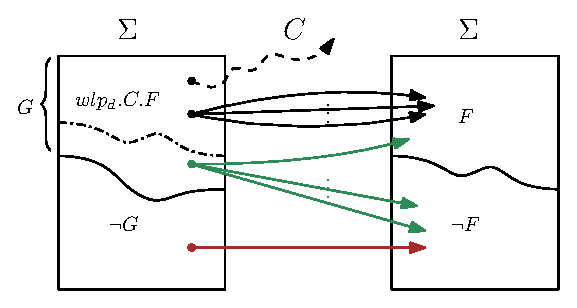
\includegraphics[width=.45\linewidth]{image/wlp-g/wlp-g-gg.eps}}
	\hfill 
	\includesvg[width=.42\linewidth]{image/wlpa.svg}
	\label{wlp-g-wlpa}
	\caption{Comparing $G$ With Angelic wlp}
\end{figure}
% However, $G$ spikes our interest when it takes the form as in \autoref{subfig:wlp-g-gg}, because under its control, the program always \imptt{can} reach a final state satisfying $F$ if it terminates, while with an initial state satisfying $\neg G$, the program is \imptt{will} terminate satisfying $\neg F$. 
% This behavior is exactly the behavior of wlp, if we were to regard the non-deterministic choice as angelic, as hinted by the similarities between \autoref{subfig:wlp-g-gg} and \autoref{subfig:wp-angelic}. 


Describing the intended behavior of wlp with angelic non-determinism (denoted by \define{wlp$_a$}) as ``if $C$ starts in an initial state satisfying $wlp_a.C.F$, then its execution either never terminates, or is always possible to end in a state satisfying $F$'', then we can deduce its semantics as follows, recalling the representation for non-termination mentioned in \autoref{sec:big-step}: 
\begin{statement}{wlpa-sound}[Semantics of $wlp_a$]%TODO
\ \vspace{-1.5mm}
\[
WRONG!!! wlp_a.C.F = \{ \sigma\in\S \mid
\neg(\exists \tau\in\S: \sigma\goto{C}\tau) \ \ \vee\ \ 
(\exists \tau\in\S: \sigma\goto{C}\tau\wedge  \tau\vDash F)
 \}
\]
% \label{thm:wlpa}
\end{statement}

While trying to distinguish what is and is not in $wlp_a$, we approach it in two directions: first, we find restraints that make the necessary liberal precondition $G$ where $wlp.C.F\implies G$ an overapproximation of angelic wlp ($ wlp_a.C.F \implies G$); then we find restraints that makes $G$ an underapproximation of angelic wlp. 
Finally, we combine both directions and conclude with statements that make $G$ and $wlp_a.C.G$ equivalent. 
We also gain a side effect of expressing wlp$_a$ without having to define it. 

\begin{lemma}{wlpa-g}[Angelic wlp implies G]
\ \\ \vspace{-3mm}
	\[\hspace{-2mm}
	\text{ if \ \ \ \ } 
	(wlp.C.F\implies G)
	\ \wedge\ 
	(sp.C.\neg G \implies \neg F) 
	\text{\ \ \ \  then\ \ \ \  } 
	wlp_a.C.F \implies G
	\] 
	\label{lem:wlp-g}
\end{lemma}
The second prerequisite \mathl{sp.C.\neg G \implies \neg F } states that from $\neg G$ we are only allowed to reach $\neg F$, making sure that all green arrows as in \autoref{fig:wlp-g-1} are included in $G$. 

% macros for referencing to lines in this chapter
\newcommand{\lblth}[1]{\hypertarget{3.#1}{{\text{#1}}}}
\newcommand{\refth}[1]{\hyperlink{3.#1}{{\text{Line (#1)}}}}
\begin{proof}
	The assumption expresses that for any state $\sigma\in\S$:
\begin{align*} 
	wlp.C.F\implies G\  \Leftrightarrow&\ \sigma\in wlp.C.F \implies \sigma\in G \\
	\Leftrightarrow&\ ( \forall \tau\in\S:\ \sigma\goto{C}\tau\implies  \tau\in F) \implies \sigma\in G \tag*{$\mid$ \thm{wlp-sound}} \\
	\Leftrightarrow&\ (\forall \tau\in\S:\ \neg(\sigma\goto{C}\tau)\ \vee\ \tau\in F) \implies \sigma\in G \\
	\Leftrightarrow&\ \neg(\exists\tau\in\S:(\sigma\goto{C}\tau)\ \wedge\ \neg(\tau\in F)) \implies \sigma\in G \tag{\lblth{a}} \\
	% && \mid \lblth{a} \\
	% &\ \ \ \  \vee (\forall \tau.\sigma\goto{C}\tau:\tau\in F \Longrightarrow \sigma\in G) 
		% \hspace{0.017\textwidth} \mid \lblth{b} \\
	%
\end{align*}
Also, for any state $\tau\in\S$: 
\begin{align*}
	sp.C.\neg G \implies \neg F \Leftrightarrow&\ \tau\in sp.C.\neg G \implies \tau\in \neg F \\
	\Leftrightarrow&\  (\exists \mu\in\S:\ \mu\goto{C}\tau\ \wedge\ \mu\in\neg G )\implies \tau\in\neg F \tag*{$\mid$ \thm{sp-sound}}\\
	% &\hspace{0.45\textwidth} \mid \thm{sp-sound}\\
	\Leftrightarrow&\  \neg (\tau\in\neg F) \implies \neg (\exists \mu\in\S:\ \mu\goto{C}\tau\ \wedge\ \mu\in\neg G ) \\
	\Leftrightarrow&\  \tau\in F \implies \forall \mu\in\S:\ \neg (\mu\goto{C}\tau\ \wedge\ \mu\in\neg G)\\
	\Leftrightarrow&\  \tau\in F \implies \forall \mu\in\S:\ \neg (\mu\goto{C}\tau)\ \vee\ \neg(\mu\in\neg G)\\
	\Leftrightarrow&\  \tau\in F \implies \forall \mu\in\S:\ \neg (\mu\goto{C}\tau)\ \vee\ \mu\in G
	\tag{\lblth{b}} \\
	%
\end{align*}
Our goal is to prove that for any state $\sigma\in\S$:
\begin{align*}
	wlp_a.C.F \implies G \Leftrightarrow&\ \sigma\in wlp_a.C.F \implies \sigma\in G \\
	\Leftrightarrow&\  \neg(\exists \tau\in\S: \sigma\goto{C}\tau) \ \vee\ 
	(\exists \tau\in\S: \sigma\goto{C}\tau\wedge  \tau\in F)\\
	&\ \ \ \ \implies \sigma\in G \tag*{$\mid$ \stm{wlpa-sound}}\\
	% &\hspace{0.45\textwidth} \mid \stm{wlpa-sound}\\
	\Leftrightarrow&\  (\neg(\exists \tau\in\S: \sigma\goto{C}\tau)\implies \sigma\in G ) \tag{\lblth{c}}\\
	% && \mid \lblth{c}\\
	&\ \wedge\ ((\exists \tau\in\S: \sigma\goto{C}\tau\wedge  \tau\in F)\implies\sigma\in G) \tag{\lblth{d}}\\
	% && \mid \lblth{d}
\end{align*}
We can prove \lem{wlpa-g} by proving that \refth{a} implies \refth{c} and that \refth{b} implies \refth{d}.
For any state $\sigma\in\S$, we first prove (a)$\implies$(c):
\begin{align*}
	% \text{(a)}\implies\text{(c)}:\text{ for any } \\
	true 
	\Leftrightarrow&\ (\exists\tau\in\S:(\sigma\goto{C}\tau)\ \wedge\ \neg(\tau\in F)) \implies (\exists\tau\in\S:\sigma\goto{C}\tau)\\ 
	\Leftrightarrow&\ \neg(\exists\tau\in\S:\sigma\goto{C}\tau) \implies \neg(\exists\tau\in\S:(\sigma\goto{C}\tau)\ \wedge\ \neg(\tau\in F))  \\ 
	\Rightarrow&\ \neg(\exists\tau\in\S:\sigma\goto{C}\tau) \implies \sigma\in G \tag*{$\mid$ \refth{a}}\\
\end{align*}
It is also valid that for any state $\sigma\in\S$, (b)$\implies$(d). 
Assume there exists $\tau\in\S$ such that for some state $\sigma\in\S$, 
$$\sigma\goto{C}\tau\ \wedge\  \tau\in F \text{ is valid. }$$
Then we conclude from \refth{b} that 
$$\forall \mu\in\S:\ \neg (\mu\goto{C}\tau)\ \vee\ \mu\in G$$
Since $\sigma\in\S$, it follows that $\neg(\sigma\goto{C}\tau)\ \vee\ \sigma\in G$. 
We already know that $\sigma\goto{C}\tau$, hence $\sigma\in G$ must be true, therefore proving \refth{d}. 
\end{proof}

Now that we can use $G$ to overapproximate $wlp_a$, the logcial next step is to underapproximate it, so that in the final step we can establish equivalences between $G$ and angelic wlp:
\begin{lemma}{g-wlpa}[G implies angelic wlp]
\ \\ \vspace{-3mm}
	\[%\hspace{-5mm}
	\text{ if \ \ \ \ } 
	(P{\implies} G) \implies \neg(sp.C.P {\implies} \neg F)
	\text{\ \ \ \  then\ \ \ \  } 
	G {\implies} wlp_a.C.F
	\] 
\end{lemma}
Here, the prerequisite states that looking at any predicate $P$ stronger than $G$ (or any subset of $G$, if we view predicates as sets of all states that satisfy them), there are no executions reaching a final state satisfying $\neg F$. 
Remember that $sp.C.P$ is exactly satisfied by states that can be reached starting from an initial state in $P$, recalling \autoref{subfig:spa}. 
The implication $sp.C.P \implies \neg F$ means that from $P$, we can \imptt{only} reach states satisfying $\neg F$. 
By negating this condition, we assert that starting from a state satisfying $P$, we should be able to reach final states other than those satisfying $\neg F$. 

Since $P$ can be singleton, i.e. a condition that is satisfied by only one state $\sigma$, then from $\sigma$ we are not allowed to \imptt{only} have executions that end in a state satisfying $\neg F$. 
Consequently, we do not allow executions starting from $G$ that \imptt{only} finish in $\neg F$, making sure that $G$ does not include the red arrows as in \autoref{fig:wlp-g-1}.  

\begin{proof}
	The assumption expresses that for any state $\sigma\in\S$:
\begin{align*} 
	&\ P\implies G \implies \neg(sp.C.P \implies \neg F) \\ 
	\Leftrightarrow&\ P\implies G \implies \neg(\forall\tau\in\S:\tau\in sp.C.P{\implies}\tau\in\neg F) \\ 
	\Leftrightarrow&\ P\implies G \implies \exists\tau\in\S:\neg(\tau\in sp.C.P{\implies}\tau\in\neg F) \\ 
	\Leftrightarrow&\ P\implies G \implies \exists\tau\in\S:\tau\in sp.C.P\ \wedge\ \neg(\tau\in\neg F) \\ 
	\Leftrightarrow&\ P\implies G \implies \exists\tau\in\S:\tau\in sp.C.P\ \wedge\ \tau\in F \\ 
	\Leftrightarrow&\ P\implies G \implies \exists\tau\in\S:(\exists \mu\in\S:\ \mu\goto{C}\tau\ \wedge\ \mu\in P)\ \wedge\ \tau\in F \tag*{$\mid$ \thm{sp-sound}}\\ 
	\Leftrightarrow&\ \sigma\in P {\implies} \sigma\in G {\implies} \exists\tau\in\S:(\exists \mu\in\S:\ \mu\goto{C}\tau\ \wedge\ \mu\in P)\ \wedge\ \tau\in F \tag{\lblth{e}}\\ 
	%
\end{align*}
Our goal is to prove that for any state $\sigma\in\S$:
\begin{align*}
	&\ G\implies wlp_a.C.F \\ 
	\Leftrightarrow&\  \sigma\in G\implies\sigma\in wlp_a.C.F\\
	\Leftrightarrow&\ \sigma\in G\implies \neg(\exists \tau\in\S: \sigma\goto{C}\tau) \ \vee\ 
	(\exists \tau\in\S: \sigma\goto{C}\tau\wedge  \tau\in F) \tag*{$\mid$ \stm{wlpa-sound}}\\
\end{align*}
For some state $\sigma\in\S$, assume $\sigma\in G$, then we can construct set $P=\{\sigma\}$ such that the prerequisites in \refth{e} holds. 
Consequently, the postrequisite in holds. 
Now we can find witnesses $\mu$ and $\tau$ such that
$$
\mu\goto{C}\tau\ \wedge\ \mu\in P\ \wedge\ \tau\in F 
$$
Since $P$ is a singleton set, $\mu$ can only be $\sigma$. 
Then we have found a witness $\tau$ such that $\sigma\goto{C}\tau$ and $\tau\in F$, satisfying the postrequisite of our goal. 
\end{proof}

\begin{corollary}{g=wlp}[G equivalent to angelic wlp]
% \begin{align*}
	\ \\
	$\text{ if } \ wlp.C.F{\implies} G \ \wedge\ 
	sp.C.\neg G {\implies} \neg F 
	\ \text{ and } \ 
	P{\implies} G \implies \neg(sp.C.P {\implies} \neg F) \\
	\text{ then }\ G = wlp_a.C.F$
% \end{align*}	
\end{corollary}

With this corollary, we can identify all initial states that lead to executions terminating satisfying our given postcondition $F$, or its opposite. 
By setting the necessary liberal precondition $G$ to be equal to $wlp_a.C.F$, we make sure that $G$ is satisfied by all such states. 
If we think $F$ to be the specification for erroneous termination, then his means that $G$ is concerned with \imptt{all} problematic initial states, and it is necessary to avoid $G$ to steer clear of those errors. 

To summarize this chapter, we started with the description of relations that connect the predicate transformers together, to introduce the necessary liberal precondition. 
Then we discovered that $G$ can be an indicator of ``bad'' precondition that is necessary to avoid, to successfully terminate. 
We can do it in two ways: 
\begin{enumerate}
	\item If we are sure that we captured all undesired final states in $F$, then we use the necessary liberal precondition that underapproximates (overapproximates) $wlp_a$, so that we catch as much ``bad'' initial states as possible. 
	\item If we only have limited knowledge of the erroneous final states, then we appeal to experts of the system for other potential errors in order to reach necessary liberal precondition. 
\end{enumerate}



%*****************************************
%*****************************************
%*****************************************
%*****************************************
%*****************************************
